\usepackage{tikz}
\usepackage{kotex}
\usepackage{amsmath,amsfonts,amssymb,mathrsfs,mathtools,adjustbox,float,graphicx,relsize}
\usepackage{dtk-logos}
\usepackage{xcolor}
\usepackage{setspace}
\usepackage{minted}
\usepackage{expl3}
\usepackage{xparse}
\usepackage{enumitem}
\usepackage{forloop}
\usefonttheme[onlymath]{serif}

\AtBeginSection[]{
  \begin{frame}
  \vfill
  \centering
  \begin{beamercolorbox}[sep=8pt,center,shadow=false,rounded=true]{title}
    \usebeamerfont{title}\insertsectionhead\par%
  \end{beamercolorbox}
  \vfill
  \end{frame}
}

\setlist[itemize,1]{label=\usebeamerfont*{itemize item}%
  \usebeamercolor[fg]{itemize item}
  \usebeamertemplate{itemize item}}
\setlist[itemize,2]{label=\usebeamerfont*{itemize subitem}%
  \usebeamercolor[fg]{itemize subitem}
  \usebeamertemplate{itemize subitem}}
\setlist[itemize,3]{label=\usebeamerfont*{itemize subsubitem}%
  \usebeamercolor[fg]{itemize subsubitem}
  \usebeamertemplate{itemize subsubitem}}
\AtBeginEnvironment{minted}{\singlespacing\fontsize{9}{12}\selectfont}
\newminted{latex}{breaklines=true,breaksymbolleft={}}
\usemintedstyle{manni}
\setminted{bgcolor=white!95!black}
\setmintedinline{fontsize=\small}

\setstretch{1.3}
\usetikzlibrary{shapes.geometric}

\makeatother
\setbeamertemplate{footline}
{
	\leavevmode%
	\hbox{%
		\begin{beamercolorbox}[wd=.3\paperwidth,ht=2.25ex,dp=1ex,center]{author in head/foot}%
			\usebeamerfont{author in head/foot}\insertshortauthor
		\end{beamercolorbox}%
		\begin{beamercolorbox}[wd=.6\paperwidth,ht=2.25ex,dp=1ex,center]{title in head/foot}%
			\usebeamerfont{title in head/foot}\insertshorttitle
		\end{beamercolorbox}%
		\begin{beamercolorbox}[wd=.1\paperwidth,ht=2.25ex,dp=1ex,center]{date in head/foot}%
			\insertframenumber{} / \inserttotalframenumber\hspace*{1ex}
	\end{beamercolorbox}}%
	\vskip0pt%
}

\makeatletter
\setbeamertemplate{navigation symbols}{}

\def\setfont{
    \ifPDFTeX
        \PackageError{MathLetter}{%
            PDFTeX is not allowed to set fonts!
        }{%
            Use another engine, such as XeLaTeX or LuaLaTeX.
        }
    \fi
    \setsansfont{Noto Sans CJK KR}[Scale=0.90,ItalicFont={*},ItalicFeatures={FakeSlant=.167}]
    \setmainhangulfont[Scale=0.90]{Noto Serif CJK KR}
    \setmainhangulfont
        [Scale=0.90,ItalicFont={*},ItalicFeatures={FakeSlant=.167}]
        {Noto Serif CJK KR}
    \setsanshangulfont[Scale=0.90]{Noto Sans CJK KR}
    \setsanshangulfont
        [ItalicFont={*},ItalicFeatures={FakeSlant=.167}]
        {Noto Sans CJK KR}[Scale=0.90]
    \setmonohangulfont{Noto Sans Mono CJK KR}
    \setmonohangulfont
        [Scale=0.90,ItalicFont={*},ItalicFeatures={FakeSlant=.167}]
        {Noto Sans Mono CJK KR}
}

\setfont


% setting some colors for the theme
\setbeamercolor{palette primary}{fg=black,bg=white}
\setbeamercolor{palette secondary}{fg=black,bg=white}
\setbeamercolor{structure}{fg=black,bg=white}
\setbeamercolor{title in head/foot}{fg=black,bg=white}
\setbeamercolor{date in head/foot}{fg=black,bg=white}



% definition of the title page template
\defbeamertemplate*{title page}{mytheme}[1][]
{%
  \begin{tikzpicture}[remember picture,overlay]
  \filldraw[white]
    (current page.north west) --
    (current page.north east) --
    ([xshift=0cm,yshift=-2cm]current page.north east)  --
    ([xshift=0cm,yshift=-2cm]current page.north west) -- cycle
    ;
   \node[opacity=0.4] at (current page.center) 
    {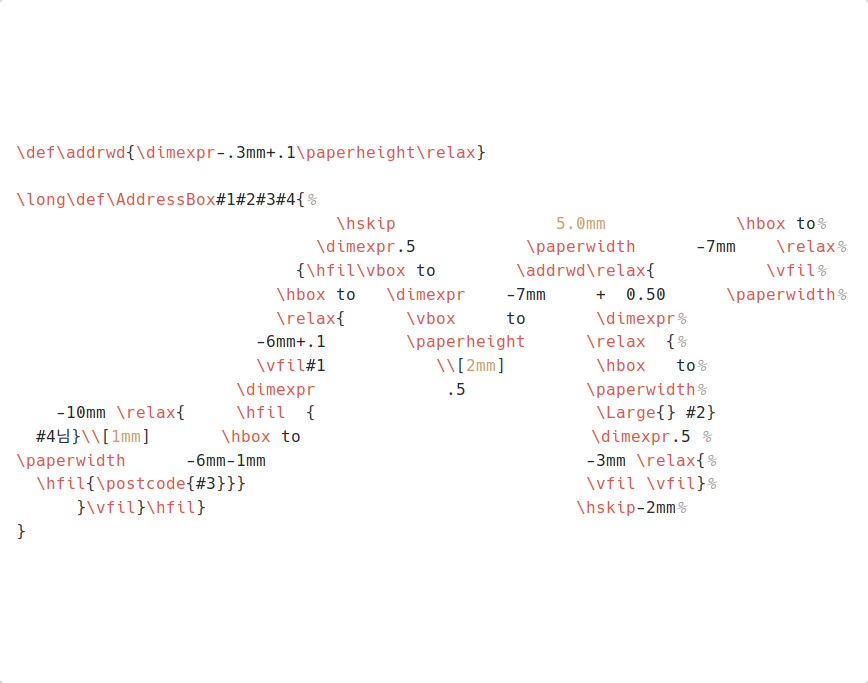
\includegraphics[scale=0.4]{msquare}};
  \node[text=black,anchor=center,font=\sffamily\LARGE,text width=\paperwidth] 
  at (current page.center)
  (title)
  {\begin{center}\inserttitle\end{center}};
    
    \node[text=black,anchor=south west,font=\sffamily\small,text width=.6\paperwidth] 
  at ([xshift=-100pt,yshift=-1.5cm]current page.center)
  (institute)
  {\raggedright\insertinstitute};
   
  \node[anchor=west]
  at ([xshift=-100pt,yshift=1cm]current page.south east)
  {};
  \node[text=black,font=\large\sffamily,anchor=south west]
  at ([xshift=30pt,yshift=0.5cm]current page.south west)
  (date)
  {\insertdate};
  \node[text=black,font=\large\sffamily,anchor=south west]
  at ([yshift=5pt]date.north west)
  (author)
  {\insertauthor};
  \end{tikzpicture}%
}

% remove navigation symbols
\setbeamertemplate{navigation symbols}{}

\definecolor{color0}{HTML}{FEABB7}
\definecolor{color1}{HTML}{9797B9}
\definecolor{color2}{HTML}{4B7AA3}

% definition of the symbols used in itemize
\newcommand\mysymbol{%
  
\begin{tikzpicture}[xscale=0.85]
    \draw (1.75ex,0) node[star, star points=5, star point ratio=2.25, inner sep=1.3pt,anchor=outer point 3,fill=color0] {};          
  \end{tikzpicture}%
}
\newcommand\mysymboli{%
  
\begin{tikzpicture}[xscale=0.85]
    \draw (1.75ex,0) node[star, star points=5, star point ratio=2.25, inner sep=1.3pt,anchor=outer point 3,fill=color1] {};          
  \end{tikzpicture}%
}
\newcommand\mysymbolii{%
  
\begin{tikzpicture}[xscale=0.85]
    \draw (1.75ex,0) node[star, star points=5, star point ratio=2.25, inner sep=1.3pt,anchor=outer point 3,fill=color2] {};          
  \end{tikzpicture}%
}

% definition of the itemize templates
\defbeamertemplate*{itemize item}{mysymbol}{\small\raise-0.5pt\hbox{\mysymbol}}
\defbeamertemplate*{itemize subitem}{mysymbol}{\footnotesize\raise-0.5pt\hbox{\mysymboli}}
\defbeamertemplate*{itemize subsubitem}{mysymbol}{\footnotesize\raise-0.5pt\hbox{\mysymbolii}}

\makeatletter
\newlength{\raising}
\newcommand{\MSquare}[1][1]{\colorlet{currentcolor}{.}\setlength{\raising}{-1pt*\ratio{\f@size pt}{5.5pt}}\edef\xscaleFactor{(0.026 * \f@size)}\edef\yscaleFactor{(-1 * \xscaleFactor)}%
\raisebox{\raising}{\begin{tikzpicture}[y=0.80pt, x=0.80pt, yscale=\yscaleFactor, xscale=\xscaleFactor, inner sep=0pt, outer sep=0pt]
\begin{scope}[shift={(0,-229.26665)},xscale=#1,yscale=#1]
\path[line width=0.065pt,fill=currentcolor] (60.5716,281.9345) -- (61.5507,279.9761) .. controls
(62.2579,278.6162) and (62.9515,277.1474) .. (63.6315,275.5699) .. controls
(64.3114,273.9923) and (65.0458,272.1972) .. (65.8346,270.1845) .. controls
(66.6233,268.1717) and (67.2353,266.6758) .. (67.6705,265.6966) .. controls
(71.0976,257.4825) and (74.0623,251.6891) .. (76.5646,248.3165) .. controls
(78.0877,246.1949) and (79.6109,244.5902) .. (81.1340,243.5023) .. controls
(83.1467,242.0335) and (84.3163,242.4959) .. (84.6427,244.8894) .. controls
(84.7515,245.7054) and (84.6971,247.2557) .. (84.4795,249.5404) .. controls
(84.2619,251.3356) and (83.9763,253.2259) .. (83.6227,255.2114) .. controls
(83.2691,257.1969) and (82.8204,259.4409) .. (82.2764,261.9432) .. controls
(81.7324,264.4455) and (81.3516,266.3222) .. (81.1340,267.5734) .. controls
(79.9373,273.5571) and (79.7469,278.9969) .. (80.5628,283.8928) .. controls
(80.9980,287.1567) and (82.1132,289.7949) .. (83.9083,291.8077) .. controls
(84.2347,292.1341) and (84.4523,292.3789) .. (84.5611,292.5420) .. controls
(84.9963,293.1948) and (85.0235,293.7932) .. (84.6427,294.3372) .. controls
(84.2075,294.8268) and (83.6363,294.8812) .. (82.9291,294.5004) .. controls
(82.2764,294.1740) and (81.7596,293.7388) .. (81.3788,293.1948) .. controls
(78.7133,289.6590) and (76.9454,285.4431) .. (76.0750,280.5473) .. controls
(75.4766,276.9026) and (75.5038,272.5508) .. (76.1566,267.4918) .. controls
(76.3742,265.8598) and (76.7550,263.5615) .. (77.2989,260.5968) .. controls
(77.8429,257.6321) and (78.2237,255.4698) .. (78.4413,254.1099) .. controls
(78.7133,252.1515) and (78.7133,250.4108) .. (78.4413,248.8877) .. controls
(78.2237,249.2140) and (77.9245,249.7308) .. (77.5437,250.4380) .. controls
(77.1629,251.1452) and (76.8910,251.6619) .. (76.7278,251.9883) .. controls
(74.3343,256.2314) and (71.6416,261.9704) .. (68.6497,269.2053) .. controls
(65.9842,275.5155) and (64.3794,279.1601) .. (63.8354,280.1393) .. controls
(61.9859,283.5120) and (60.0820,285.7967) .. (58.1236,286.9935) .. controls
(57.5797,287.3198) and (57.1717,287.1838) .. (56.8997,286.5855) .. controls
(55.3765,283.0496) and (54.7238,279.5681) .. (54.9414,276.1411) .. controls
(54.9958,275.1619) and (55.1454,273.7611) .. (55.3901,271.9388) .. controls
(55.6349,270.1165) and (55.7845,268.8517) .. (55.8389,268.1446) .. controls
(55.9477,266.9478) and (56.1925,264.9351) .. (56.5733,262.1064) .. controls
(56.9541,259.2777) and (57.1989,257.1018) .. (57.3077,255.5786) .. controls
(57.5797,252.6955) and (57.7157,250.1116) .. (57.7157,247.8269) --
(57.7157,247.0109) -- (57.4709,247.0109) .. controls (55.4037,250.3836) and
(53.6358,254.1371) .. (52.1671,258.2713) .. controls (49.7736,265.1799) and
(47.8968,269.9941) .. (46.5369,272.7140) .. controls (43.9258,277.9362) and
(40.7163,281.6896) .. (36.9084,283.9744) .. controls (33.8077,285.8783) and
(30.3535,287.0478) .. (26.5456,287.4830) .. controls (23.4993,287.8094) and
(20.6434,287.9454) .. (17.9779,287.8910) .. controls (12.4837,287.6734) and
(8.4039,287.1294) .. (5.7384,286.2591) .. controls (4.7592,285.9327) and
(3.7800,285.4703) .. (2.8009,284.8719) .. controls (0.5162,283.4576) and
(0.1626,281.6624) .. (1.7401,279.4865) .. controls (2.7737,278.0722) and
(4.4872,276.6578) .. (6.8807,275.2435) .. controls (10.6886,273.0132) and
(15.5028,271.0004) .. (21.3234,269.2053) .. controls (27.6336,267.3014) and
(33.9981,265.8326) .. (40.4171,264.7991) .. controls (41.5051,264.5815) and
(42.3754,264.4999) .. (43.0282,264.5543) .. controls (43.5178,264.6631) and
(43.8714,264.8807) .. (44.0890,265.2071) .. controls (44.1978,265.5334) and
(44.0618,265.8870) .. (43.6810,266.2678) .. controls (43.1370,266.8662) and
(41.9946,267.5734) .. (40.2539,268.3893) .. controls (37.2620,269.5861) and
(32.1214,271.0276) .. (24.8321,272.7140) .. controls (17.8147,274.3459) and
(13.1909,275.5699) .. (10.9606,276.3858) .. controls (7.9143,277.5826) and
(5.7384,278.7793) .. (4.4328,279.9761) .. controls (3.5625,280.6833) and
(3.1817,281.2545) .. (3.2905,281.6896) .. controls (3.3449,281.9616) and
(3.4673,282.1384) .. (3.6577,282.2200) .. controls (3.8480,282.3016) and
(4.1200,282.3696) .. (4.4736,282.4240) .. controls (4.8272,282.4784) and
(5.0312,282.5056) .. (5.0856,282.5056) .. controls (5.6840,282.6144) and
(8.5399,282.8048) .. (13.6533,283.0768) .. controls (16.6996,283.1856) and
(20.3442,283.1584) .. (24.5873,282.9953) .. controls (29.1567,282.7777) and
(32.6654,282.1521) .. (35.1133,281.1186) .. controls (38.5948,279.6498) and
(41.4235,276.9299) .. (43.5994,272.9589) .. controls (44.6329,271.1637) and
(46.1017,267.4919) .. (48.0056,261.9433) .. controls (50.0727,256.0683) and
(51.7319,252.0428) .. (52.9830,249.8669) .. controls (54.6150,247.0382) and
(56.4101,244.7535) .. (58.3684,243.0128) .. controls (58.9668,242.4688) and
(59.6468,242.0336) .. (60.4084,241.7072) .. controls (61.5507,241.2720) and
(62.2851,241.5984) .. (62.6115,242.6864) .. controls (62.8835,243.6111) and
(63.0739,244.7263) .. (63.1827,246.0319) .. controls (63.3459,250.3837) and
(62.9923,255.5243) .. (62.1219,261.4537) .. controls (60.9795,269.6134) and
(60.3540,274.2916) .. (60.2452,275.4884) .. controls (60.0820,277.6099) and
(60.1092,279.5954) .. (60.3268,281.4450) .. controls (60.2724,281.6081) and
(60.3540,281.7713) .. (60.5716,281.9345) -- cycle(93.0472,250.7644) --
(99.0038,250.7644) .. controls (99.6565,250.7100) and (100.0917,250.8324) ..
(100.3093,251.1316) .. controls (100.5269,251.4308) and (100.6357,251.9067) ..
(100.6357,252.5595) .. controls (100.6357,252.9947) and (100.6085,253.3347) ..
(100.5541,253.5795) .. controls (100.4997,253.8243) and (100.3501,254.0283) ..
(100.1053,254.1915) .. controls (99.8605,254.3547) and (99.4933,254.4363) ..
(99.0038,254.4363) .. controls (95.6311,254.3819) and (92.2584,254.3819) ..
(88.8857,254.4363) .. controls (87.7978,254.4363) and (87.3626,253.9467) ..
(87.5802,252.9675) .. controls (87.9066,251.0092) and (88.8857,249.2412) ..
(90.5177,247.6637) .. controls (91.0073,247.2829) and (91.7280,246.6845) ..
(92.6800,245.8686) .. controls (93.6320,245.0526) and (94.3527,244.4270) ..
(94.8423,243.9918) .. controls (95.9847,243.0671) and (96.4743,241.8703) ..
(96.3111,240.4016) .. controls (96.0935,239.0416) and (95.4679,238.3072) ..
(94.4343,238.1985) .. controls (93.1288,238.0353) and (92.2584,238.6336) ..
(91.8232,239.9936) .. controls (91.7688,240.1024) and (91.7417,240.3064) ..
(91.7417,240.6056) .. controls (91.7417,240.9048) and (91.7009,241.1495) ..
(91.6193,241.3399) .. controls (91.5377,241.5303) and (91.3881,241.6527) ..
(91.1705,241.7071) .. controls (90.5721,241.9247) and (89.6473,241.9247) ..
(88.3962,241.7071) .. controls (87.8522,241.6527) and (87.6618,241.2719) ..
(87.8250,240.5648) .. controls (87.9338,239.3136) and (88.3554,238.1440) ..
(89.0897,237.0561) .. controls (89.8241,235.9681) and (90.7081,235.2609) ..
(91.7417,234.9346) .. controls (94.6791,234.0642) and (97.0726,234.7170) ..
(98.9222,236.8929) .. controls (100.7173,238.9600) and (101.0437,241.2447) ..
(99.9013,243.7470) .. controls (99.3574,244.9438) and (98.5414,245.9502) ..
(97.4534,246.7661) .. controls (96.9639,247.0925) and (95.4679,248.3165) ..
(92.9656,250.4380) .. controls (92.9656,250.5468) and (92.9928,250.6556) ..
(93.0472,250.7644) -- cycle;
\end{scope}
\end{tikzpicture}}}
\makeatother


\title[2019 편집부 \LaTeX\ 세미나]{\bf2019 편집부 \LaTeX\ 세미나}
\author{\MSquare\ 편집부장 김기택 \smaller(제작 김건우)}
\date{}

\institute{}
